% LyX 2.1.1 created this file.  For more info, see http://www.lyx.org/.
%% Do not edit unless you really know what you are doing.
%\documentclass[letterpaper,twocol,amsmath,aps,jcp,preprintnumbers,groupaddress,nofootinbib,tightenlines]{revtex4-1}
%\usepackage[latin9]{inputenc}
%\usepackage{textcomp}

\documentclass[letterpaper,twocolumn,amsmath,amsfont,amssymb,english,aps,jcp,preprintnumbers,groupaddress,nofootinbib,tightenlines]{revtex4}

\usepackage{graphicx}


%\documentclass[aps,prb,letterpaper,twocolumn,nofootinbib,showkeys]{revtex4-1}
%\documentclass[aps,amssymb,prl,letterpaper,twocolumn,nofootinbib,showkeys]{revtex4-1}

%\usepackage[backend=bibtex]{biblatex}

%    backend=biber,
%    style=authoryear,
%    natbib=true,
%    sortlocale=en_US,
%    url=false,
%    doi=true,f
%    eprint=false
%]{biblatex}
%\usepackage{hyperref}


\newcommand{\mat}[1]{\boldsymbol{#1}}
\newcommand{\matT}[1]{\boldsymbol{#1}^\dagger}
\newcommand{\ot}{ {\scriptstyle \otimes}_{ \tau } }

%%\hypersetup{pdftitle={FreeON Project Report 1}}
%\hypersetup{pdfauthor={Matt Challacombe and Nicolas Bock}}
%\hypersetup{pdfsubject={A SpAMM Stabilized Newton Schulz Preconditioner: Fighting Error with Error}}

%\bibstyle{aipnum4-1}

\begin{document}

\title{On Stability of Newton Schulz Iterations in an Approximate Algebra}

\author{Matt Challacombe}
\email{matt.challacombe@freeon.org}
\homepage{http://www.freeon.org}
\affiliation{Theoretical Division, Los Alamos National Laboratory}

\author{Nicolas Bock}
\email{nicolasbock@freeon.org}
\homepage{http://www.freeon.org}
\affiliation{Theoretical Division, Los Alamos National Laboratory}

%\begin{abstract}
%Forward look
%\end{abstract}

\maketitle
\section{Introduction}

In many areas of application, finite correlations lead to matrices with decay properties.  Matrix decay involves an approximate 
(perhaps bounded \cite{}) inverse 
relationship between matrix elements and a related distance;  this may be a simple inverse exponential relationship between elements and the
Cartesian distance between support functions, or it may involve a generalized distance, {\em e.g.}~ a statistical measure between strings.  
In electronic structure,  correlations manifest in decay properties of the gap shifted matrix 
sign function, as projector of the effective Hamiltonian (Fig.~\ref{figure1}).  
More broadly, matrix decay properties may coorespond to statistical matrices 
\cite{penrose1974,voit00,Anselin2003,Hardin2013,Krishtal2014}, including learned correlations in a 
generalized, non-orthogonal metric \cite{}. More broadly still, problems with local, non-orothogonal support 
are often solved with congruential transformations of the matrix inverse square root \cite{Lowdin56,naidu11} or a related factorization \cite{Krishtal2014};
these transformations correlate local support with a representation independent form, {\em eg.}~of the eigenproblem. 
Interestingly, the matrix sign function and the matrix inverse square root function are related by Higham's identity:
\begin{equation}
\rm{sign} \left( \begin{bmatrix} 0 & \mat{s}      \\ \mat{I}       & 0\end{bmatrix} \right)  =
                 \begin{bmatrix} 0 & \mat{s}^{1/2} \\ \mat{s}^{-1/2} & 0\end{bmatrix}  .
\end{equation}
A complete overivew of matrix function theory and computation is given in Higham's enjoyable reference \cite{Higham08}. 

A well conditioned matrix $\mat{s}$ may often correspond to matrix sign and inverse square root functions with rapid exponential decay, 
and be amenable to the sparse matrix approximation
$\bar{\mat{s}} = \mat{s}+ \mat{\epsilon}^{\mat{s}}_\tau$, where $\mat{\epsilon}^{\mat{s}}_\tau$ is the error introduced according to some  
criteria $\tau$.  Supporting this approximation are usefull bounds to matrix function elements \cite{Benzi99b, }.  
The criteria $\tau$ might be a drop-tolerence, 
$\epsilon^{\mat{s}}_{\tau} = \{-s_{ij}*\hat{\mat{e}}_i \, | \, |s_{ij}|<\tau \}$, a radial cutoff, 
$\epsilon^{\mat{s}}_{\tau} = \{-s_{ij}*\hat{\mat{e}}_i \, | \, \lVert \mat{r}_i - \mat{r}_j \rVert > \tau \}$, 
or some other approach to truncation, perhaps involving a sparsity pattern chosen {\em a priori}. 
Then, conventional computational kernels may be employed, such as the sparse general matrix-matrix multiply 
($\tt{SpGEMM}$) \cite{Gustavson78, Toledo97,challacombe00,bowler00}, yeiding fast solutions for multiplication rich iterations and a modulated fill in. 
These and related incomplete/inexact approaches to the computation of sparse approximate matrix functions often lead to ${\cal O}(n)$ 
algorithms, finding wide use in technologically important preconditioning schemes, the information sciences, electronic structure and many
other disciplines.  Comprehensive surveys of these methods in the numerical linear algebra are given by Benzi \cite{Benzi99,Benzi02}, and
by Bowler \cite{Bowler12} and Benzi \cite{Benzi13} for electronic structure.

\begin{figure}[t]\label{figure1}
 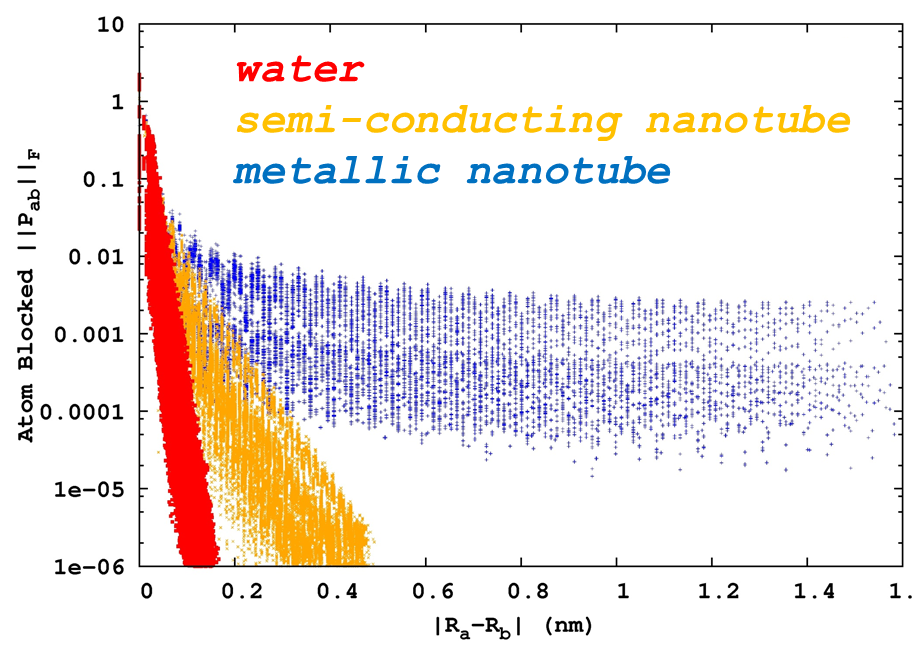
\includegraphics[width=3.5in]{decay_picture.png}
  \caption{Examples from electronic structure of decay for the spectral projector (gap shifted sign function) with respect to local (atomic) support.  
           Shown is decay for systems with correlations that are short (insulating water), medium (semi-conducting 4,3 nanotube), and 
           long (metalic 3,3 nanotube) ranged,  from exponential (insulating) to algebraic (metallic). }
\end{figure}

Because the truncated multiplication is controled only by absolute, addititve errors in the  product,   
\begin{equation}
\overline{ \mat{a} \cdot \mat{b} }\; = \; \mat{a}\cdot\mat{b} \; +\; \mat{\epsilon}^{\mat{a}}_\tau \cdot \mat{b} \;+\;
 \mat{a} \cdot \mat{\epsilon}^{\mat{b}}_\tau  \; + \;   {\mathcal O}(\tau^2)
\end{equation}
achieving sparse, stable and rapidly convergent iteration for ill-conditioned problems can be challenging \cite{}.  In cases of 
extreme degeneracy,  hierarchical semi-seperable (reduced rank) algorithms  can offer effective complexity reduction \cite{}.
However, many pratical cases are somewhere in-between sparse and meaningfully degenerate regimes; effectively dense but without
an exploitable reduction in rank.  This is the case in electronic structure for strong but non-metalic correlation, 
{\em e.g.}~towards the Mott transition \cite{}, and also in the case of local atomic support towards completeness \cite{Others, Hutter, Gigi}. 

\pagebreak
In this contribution, we consider an $N$-body approach to the approximation of matrix functions with decay, 
based on the quadtree \cite{wise, samet} 
\begin{equation}
\mat{a}^i = \begin{bmatrix} \,  \mat{a}^{i+1}_{00} \, & \,  \mat{a}^{i+1}_{01} \,  \\[0.2cm]  \, \mat{a}^{i+1}_{10} \,  & \,\mat{a}^{i+1}_{11} \, \end{bmatrix} \, ,
\end{equation}
and orderings that are locality preserving \cite{}.  Orderings that preserve data locality are well developed in the
spatial and metric database theory \cite{}, are the cornerstone of $N$-Body methods \cite{}, and an increasingly important problem 
for runtime systems, with memory hierarchies becoming increasingly assynchronous and decentralized \cite{cache}.  
Orderings that enhance locality lead  ideally to  block-by-magnitude matrix structures, with well segregated blocks 
of like size.  Perhaps the most effective approaches to data locality employ Space filling curve (SFC) heuristics to order the 
Cartesian positions of local support functions, such as finite elements (FEMs) \cite{} and atomic basis functions (LCAOs) \cite{}.

The data local approach is distinct from sparse radomized methods for the high performance $\tt SpGEMM$ that enjoy work load 
homogenisation and conventional (dense) communication strategies \cite{}.   Tradinng irregularity for homogenaity, the data-centric 
methods enable fast range and metric querries that support local approximation \cite{}.

and associated algorithms \cite{samet}.  
The Sparse Approximate Matrix Multiplication ($\tt SpAMM$) kernel, $\ot$, 
employs 

metric querry on sub-multiplicative norms to achieve a reduced ${\cal O}(n)$ cost for occlusion of 
terms through recursive application of the Cauchy-Schwarz inequality \cite{}, 
\begin{widetext}
\begin{equation}
\mat{a}^{i} \ot \mat{b}^{i} = 
\left\{
        \begin{array}{ll}
                 \emptyset \quad \tt{if}\quad \lVert \mat{a}^i \rVert \lVert \mat{b}^i \rVert < \tau \\[0.2cm]
                 \mat{a} ^i \cdot \mat{b}^i \quad  \tt{if}(i=\tt{leaf}) \\[0.2cm]
\begin{bmatrix} \mat{a}^{i+1}_{00} \ot \mat{b}^{i+1}_{00} +\mat{a}^{i+1}_{01} \ot \mat{b}^{i+1}_{10} \; , \; &
                \mat{a}^{i+1}_{00} \ot \mat{b}^{i+1}_{01} +\mat{a}^{i+1}_{01} \ot \mat{b}^{i+1}_{11}  \\[0.2cm] 
                \mat{a}^{i+1}_{00} \ot \mat{b}^{i+1}_{01} +\mat{a}^{i+1}_{01} \ot \mat{b}^{i+1}_{11} \; , \; & 
                \mat{a}^{i+1}_{00} \ot \mat{b}^{i+1}_{01} +\mat{a}^{i+1}_{01} \ot \mat{b}^{i+1}_{11}   
\end{bmatrix}  \quad \tt{else}
                \end{array}
              \right.  \, ,
\end{equation}
\end{widetext}
with $\lVert \cdot \rVert \equiv \lVert \cdot \rVert_F$ because computability \cite{kahan}.  In addition to the potential for 
${\cal O}(n)$ cost, the $N$-Body approach to the linear algebra of matrices with decay offers the potential for generic high 
performance implementations and strong parallel scaling \cite{},  
improved error accumulation relative to row-col contraction \cite{}, and a simple, intuiative code base \cite{}.  
Perhaps most importantly though, the occlusion error 

at recursively fine levels of granularity,
and supporting both sparse \cite{wise} and compressive \cite{} approaches to linear algebra.   
With decay and matrix quadtrees structured block-by-magnitude, 






\begin{equation}
\mat{\Delta}^{a\cdot b}_{\tau}=\mat{a} \ot \mat{b}-\mat{a}\cdot \mat{b}
\end{equation}
obeys the multiplicative bound 
\begin{equation}
\lVert \mat{\Delta}^{a \cdot b}_{\tau} \rVert \, \leq \, \tau \, \lVert \mat{a} \rVert  \,  \lVert \mat{b} \rVert \, ,
\end{equation}
with the potential for {\em relative} error control during iteration.   Generally, $\ot$ yeilds a non-associative algebra with Lie bracket
\begin{equation}
\left[ \mat{a} , \mat{b} \right]_{\tau} = \mat{a} \ot \mat{b}-\mat{b} \ot \mat{a}  
=  \left[ \mat{a} , \mat{b} \right]
+ \mat{\Delta}^{a\cdot b}_{\tau} -\mat{\Delta}^{b\cdot a}_{\tau}.
\end{equation}
Here, we hope to understanding the flow of occlusion errors under Newton Schulz iteration, 
for ill-conditioned problems and with extreme permisive values of $\tau$. 

\section{Newton Shulz Iteration}

\subsection{Retaining the Eigenspace}
Gradients lack convergence properties
Iteration without orig drives away from basis
NS has both.  Difference between scalar iteration, Higham page 92.


\subsection{Idempotence }

\subsection{The Scaled Map}

\subsection{Alternative Formulations}
dual, stabilized and naive

\section{Occlusion Flows}

$\delta \mat{x}_k$ and $\delta \mat{z}_k$ arrize from itteration with $\ot$, and are deterministic 
flows away from the manifold of $\mat{s}$ determined by sensitivity of the NS iteration to these 
numerical insults. 


\begin{equation}
\delta \mat{x}^{\rm{naiv}}_k =   \delta  \widetilde{ \mat{z}}_{k} \cdot \mat{s} \cdot \widetilde{\mat{z}}_{k} 
                           +  \widetilde{\mat{z}}_{k} \cdot \mat{s} \cdot \! \delta \widetilde{\mat{z}}_{k} 
\end{equation}



\begin{equation}
\delta \mat{x}^{\rm{dual}}_k =   \delta  \widetilde{ \mat{y}}_{k} \cdot \widehat{\mat{z}}_{k} 
                           +  \widetilde{\mat{y}}_{k} \cdot \delta \widetilde{\mat{z}}_{k} 
\end{equation}


\begin{eqnarray}
\widetilde{\mat{x}}_k &=& f \left[\widetilde{\mat{z}}_{k-1} , \widetilde{\mat{x}}_{k-1} \right] \\ 
&=&
\tt{m} \left[ \widetilde{\mat{x}}_{k-1}\right] \cdot \widetilde{\mat{z}}^\dagger_{k-1}  
\cdot \mat{s} \cdot \widetilde{\mat{z}}_{k-1} \cdot \tt{m}\left[ \widetilde{\mat{x}}_{k-1} \right] 
\nonumber
\end{eqnarray}

\begin{equation}
\delta \mat{x}_k = {f}_{\delta \mat{z}_{k-1}}  \, \lVert \delta \mat{z}_{k-1} \rVert 
                              +  {f}_{\delta \mat{x}_{k-1}}   \, \lVert \delta \mat{x}_{k-1} \rVert 
                                                                                      + {\cal{O}} \left(  \tau^2 \right)
\end{equation}

generalized Gateaux differential

\begin{eqnarray}
f_{\delta \mat{z}_{k-1}} &=& \lim_{\tau \rightarrow 0} \frac{ f [ \mat{z}_{k-1} +\tau  \delta \widehat{\mat{z}}_{k-1}, \widetilde{\mat{x}}_{k-1} ]
-f [\, \mat{z}_{k-1}, \widetilde{\mat{x}}_{k-1} ]  }{\tau} \nonumber  \\[0.1cm] 
&=&{L}_{\widetilde{\mat{x}}_k}\left(\widetilde{\mat{z}}_{k} , \delta \widehat{\mat{z}}_{k-1} \right)  
\end{eqnarray}

\begin{eqnarray}
f_{\delta \mat{x}_{k-1}} &=& \lim_{\tau \rightarrow 0} \frac{ f [ \widetilde{\mat{z}}_{k-1}, \mat{x}_{k-1} + \tau \delta \widehat{\mat{x}}_{k-1} ]
-f [ \widetilde{\mat{z}}_{k-1}, \mat{x}_{k-1} ]  }{\tau} \nonumber  \\[0.1cm] 
&=&{L}_{\widetilde{\mat{x}}_k}\left(\widetilde{\mat{z}}_{k} , \delta \widehat{\mat{x}}_{k-1} \right)  
\end{eqnarray}

\begin{multline}
{L}_{\widetilde{\mat{x}}_k}\left(\widetilde{\mat{z}}_{k} , \delta \widehat{\mat{x}}_{k-1} \right) 
= \delta \widehat{\mat{x}}^\dagger_{k-1} \cdot   \tt{m}'\left[\mat{x}_{k-1} \right] \cdot 
\{\widetilde{\mat{z}}^\dagger_{k-1}  \cdot \mat{s} \cdot \widetilde{\mat{z}}_{k} \}  \\
+ \{ \widetilde{\mat{z}}^\dagger_{k} \cdot \mat{s} \cdot  \widetilde{\mat{z}}_{k-1} \} 
\cdot \tt{m}'\left[\mat{x}_{k-1} \right]  \cdot \delta \widehat{\mat{x}}_{k-1} 
\end{multline}

\begin{multline}
{L}_{\widetilde{\mat{x}}_k}\left(\widetilde{\mat{z}}_{k} , \delta \widehat{\mat{z}}_{k-1} \right) = 
\{ \tt{m}\left[\mat{x}_{k-1} \right]  \cdot \delta {\widehat{\mat{z}}}^\dagger_{k-1} 
 \cdot \mat{s} \} \cdot \widetilde{\mat{z}}_{k} \\
+\widetilde{\mat{z}}^\dagger_{k} \cdot \{ \mat{s} \cdot \delta {\widehat{\mat{z}}}_{k-1}
\cdot \tt{m}\left[\mat{x}_{k-1} \right]    \} 
\end{multline}

\begin{equation}
 \{ \widetilde{\mat{z}}^\dagger_{k} \cdot \mat{s} \cdot  \widetilde{\mat{z}}_{k-1} \} 
\rightarrow \mat{p}_+\left[\mat{s} \right]
\end{equation}

\begin{equation}
\{ \mat{s} \cdot \delta {\widehat{\mat{z}}}_{k-1}
\cdot \tt{m}\left[\mat{x}_{k-1} \right]    \} 
\rightarrow \mat{n}\left[\mat{s} \right]
\end{equation}


\section{Implementation}

\subsection{Methods}
FP, F08, OpenMP 4.0

\subsection{A Modified NS Map}

\subsection{$\delta \mat{x}_k$ and $\delta \mat{x}_k$ channels}
tau= Figure showing channels etc.  

\subsection{Convergence}
Map switching and etc based on TrX


\section{Ill-Conditioned Support}

\subsection{ 3,3 carbon nanotube with diffuse $sp$-function}
double exponential (Fig.)

\subsection{Water with triple zeta and double polarization}
Here's looking at you Jurg...

\section{Experiments}

\subsection{Occlusion Flows}
\begin{figure}[h]
  \caption{equation...}
 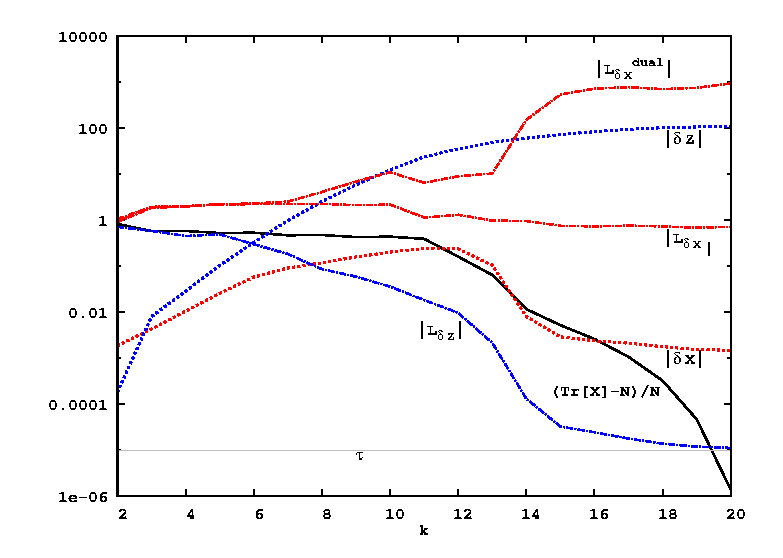
\includegraphics[width=3.5in]{8x_33_nanotube_cond10_tau-5.eps}
 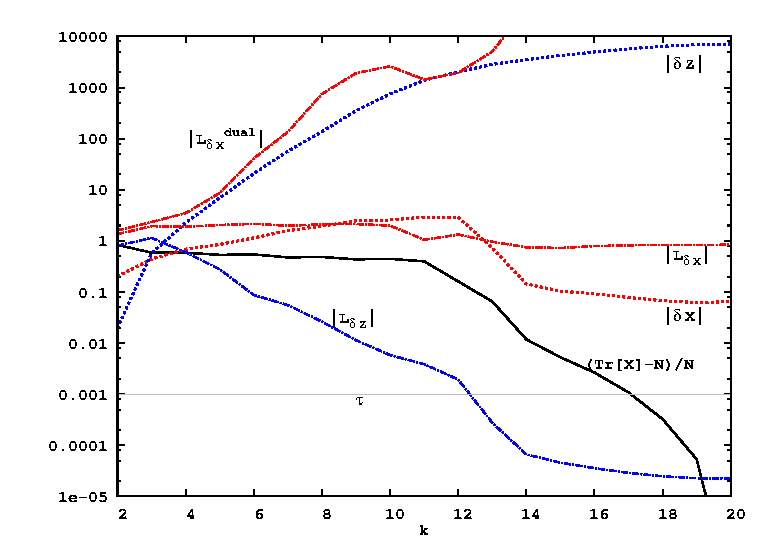
\includegraphics[width=3.5in]{8x_33_nanotube_cond10_tau-3.eps}
\end{figure}
\begin{figure}[h]
  \caption{equation...}
 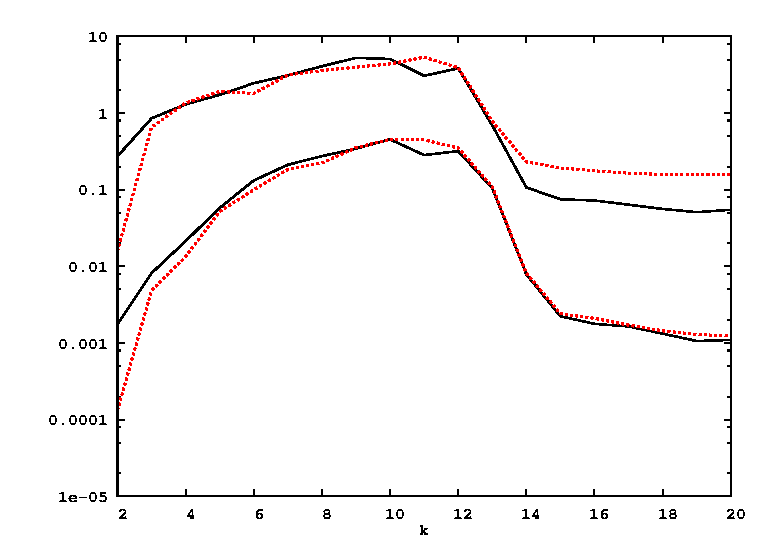
\includegraphics[width=3.5in]{8x_33_nanotube_cond10_compare_errors.eps}
\end{figure}

\subsection{Comments}

\begin{multline}
 \delta {\mat{z}}_{k-1} \approx \Delta^{\widetilde{\mat{z}}_{k-2} \cdot \tt{m}\left[ \widetilde{\mat{x}}_{k-2}\right]}_\tau 
+ \mat{z}_{k-2} \cdot \tt{m}'\left[ \widetilde{\mat{x}}_{k-2}\right] \cdot \delta \mat{x}_{k-2} \\
+\delta \mat{z}_{k-2} \cdot \tt{m} \left[\widetilde{\mat{x}}_{k-2} \right] 
\end{multline}

\begin{multline}
\lVert \delta {\mat{z}}_{k-1} \rVert \lesssim
\lVert \mat{z}_{k-2} \rVert \left( \;  \tau \, \lVert \tt{m} \left[\widetilde{\mat{x}}_{k-2} \right]  \rVert \right.   \\ \left.
+ \; \lVert \delta {\mat{x}}_{k-2} \rVert   \lVert \tt{m}' \left[\widetilde{\mat{x}}_{k-2} \right] \rVert \; \right)
\end{multline}

\begin{equation}
\lVert \mat{z}_{k} \rVert  \rightarrow \sqrt{\kappa\left(\mat{s} \right)}
\end{equation}

\subsection{Occlusion Boundaries}

\begin{figure}[h]
  \caption{equation...}
 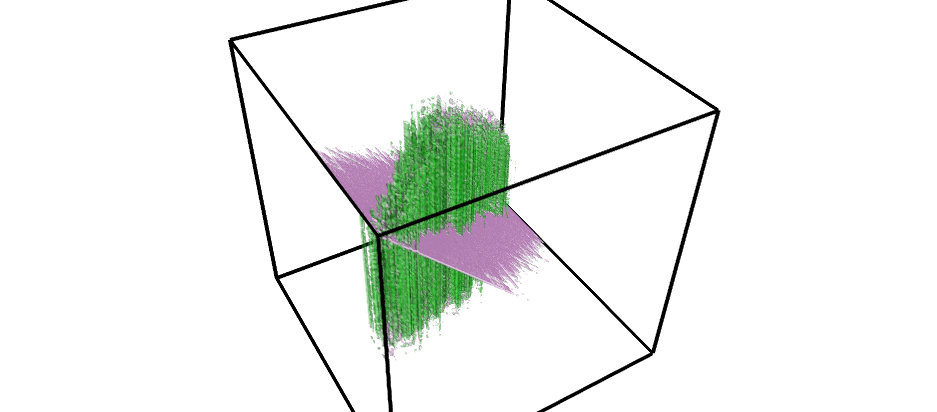
\includegraphics[width=3.5in]{snapshot.png}
\end{figure}

\subsection{Comments}

\subsection{Scaling}

\subsection{Comments}
Pictures of the spamm structure

\section{Conclusion}

%%eg vs row-col picture.  Example of exact exchange w/DBSR 

\bibliography{MatrixFunctions}

\end{document}
